% Technical report, Solar Filament Segmentation Challenge 2026 (IEEE BigData Cup).
% Written in IEEEtran conference format; move the sections into the organisers' Overleaf template.
% Figures are read from ../docs/figures (upload that folder next to this file on Overleaf).
\documentclass[conference]{IEEEtran}
\usepackage{graphicx}
\usepackage{booktabs}
\usepackage{amsmath}
\usepackage{siunitx}
\usepackage[hidelinks]{hyperref}
\graphicspath{{../docs/figures/}{figures/}}

\begin{document}

\title{A Consensus-Trained U-Net with a Learned Component Scorer for Solar Filament Instance Segmentation,\\and What Limits Panoptic Quality on MAGFiLO}

\author{\IEEEauthorblockN{Mukharbek Organokov}
\IEEEauthorblockA{[affiliation] \\ [e-mail]}}

\maketitle

\begin{abstract}
We segment solar filaments on GONG H-alpha full-disk images of the MAGFiLO dataset with a single U-Net
(ResNet-34 encoder) at 1536~px, trained on the consensus of the annotators and averaged over four flips.
Its connected components are candidates; a gradient-boosted component scorer, trained on out-of-fold
candidates, predicts each one's expected contribution to Panoptic Quality (PQ) and keeps those that pay.
On all 707 training images, scored out of fold with a split by calendar month, the pipeline reaches PQ
0.422 (segmentation quality 0.674, recognition quality 0.626), against 0.409 for the same network at
1024~px with a hand-tuned rule; the public leaderboard gives 0.35. One MAGFiLO annotator scored against
another on the same images reaches only PQ 0.340. We report the experiments that did not help (a Mask
R-CNN detector, a crop refiner, a larger encoder, limb-darkening correction, a Lov\'asz loss, ensembling,
2048~px input and seven post-processing rules) and show that most of the remaining loss is annotator
disagreement rather than model error.
\end{abstract}

\section{Introduction}
Filaments are dense, cool plasma suspended above polarity inversion lines; they appear as dark, elongated
structures in H-alpha and are at the origin of many eruptions. MAGFiLO~\cite{magfilo} provides manual
segmentations of filaments on GONG H-alpha images, with up to three independent annotators per image.
The challenge asks for one mask per filament and scores them with PQ~\cite{kirillov2019}.

The data has a property that shapes every decision: annotators disagree strongly, and each annotator is
scored separately against the same prediction. A prediction can therefore never match all annotators,
and the best achievable PQ is far below 1. Our contributions are (i) a simple and reproducible
pipeline; (ii) a component scorer that selects instances by their expected PQ contribution, which beats
the hand rules we tuned; (iii) a measurement of the annotator ceiling and an error analysis that
explains why the common improvements fail; and (iv) the negative results, reported with numbers.

\section{Data and metric}
The training set has 707 images (2048$\times$2048 px) with 8{,}199 annotated filaments; 411 images have
one annotator, 145 two and 151 three, giving 1{,}154 annotator-image entries. The test set has 180 images.
For each entry, a ground-truth (GT) and a predicted mask form a true positive (TP) when their IoU exceeds
0.5; PQ is $\sum_{TP}\mathrm{IoU} / (|TP| + 0.5|FP| + 0.5|FN|)$, pooled over all entries. It factors into
segmentation quality SQ (mean IoU of the TPs) and recognition quality RQ.

Our implementation of the metric reproduces the organisers' self-evaluation notebook exactly. Reading
that code showed that it does not enforce one-to-one matching, so two overlapping predictions of one
filament would both count as TPs. Duplicating our own confident out-of-fold masks would raise PQ from
0.409 to 0.61 without detecting anything new, since PQ then tends to the SQ of the duplicated masks.
We did not submit such files: all our submissions are disjoint by construction.

\section{Method}
\subsection{Input and target}
Each image is area-downsampled to 1536~px and normalised with fixed constants. The training target is
the consensus: the fraction of annotators marking each pixel, computed at 2048~px and then downsampled.
A network trained with binary cross-entropy (BCE) on this soft target learns the probability that an
annotator marks a pixel, which is the quantity the multi-annotator metric rewards.

\subsection{Network and training}
A U-Net~\cite{unet} from \texttt{segmentation\_models\_pytorch}~\cite{smp} with an ImageNet ResNet-34
encoder~\cite{resnet}, adapted to one input channel (24.4~M parameters). Loss: BCE + soft Dice. AdamW,
learning rate $5\cdot10^{-4}$ with one epoch of warm-up and cosine decay, weight decay $10^{-4}$, batch 4,
40 epochs. Augmentation: flips, 90-degree rotations, affine ($\pm30^\circ$, scale 0.9--1.1), brightness,
contrast and gamma. The final model is trained on all 707 images (36~min on an NVIDIA A100 via
Hugging Face Jobs; about 3~h on an Apple M3 Max).

\subsection{From probabilities to instances}
At inference the probability is averaged over four flipped views (identity, horizontal, vertical, both)
and upsampled bilinearly to 2048~px. The map is thresholded at 0.45. A morphological closing with a 31~px
disk is used only to decide which fragments belong to one filament: the scored masks keep the thresholded
pixels. The 8-connected components of at least 100~px are the candidates; they are disjoint by construction.

\subsection{Component scorer}
Every false positive costs half a point in the PQ denominator, so the choice of which candidates to submit
matters as much as their shape. A hand rule (area $\geq 300$~px and mean probability $\geq 0.8$) treats all
candidates alike. Instead, for each OOF candidate we compute the target
$y = \frac{1}{n}\sum_{e} \mathrm{IoU}_e \,[\mathrm{IoU}_e > 0.5]$ over the $n$ annotator entries $e$ of its
image, i.e.\ its expected matched IoU per entry, and regress it with a gradient-boosted tree model
(scikit-learn \texttt{HistGradientBoostingRegressor}) on 20 features: area, the mean, maximum, spread and
quantiles of the probability inside, elongation, length, width and compactness, the brightness contrast with
a 15~px ring around the component, distance from disk centre, latitude and longitude on a disk fitted with a
Hough circle, and two image-level features (number of candidates, mean probability). A candidate pays when
$y$ exceeds about PQ/2 (Section~\ref{sec:loss}); we keep candidates whose prediction exceeds $\tau=0.20$
(PQ varies by less than 0.001 over $\tau=0.15$--$0.25$). Inference, including features, takes 4.5~s per image.

\subsection{Validation and tuning}
Filaments persist for days, so images from the same week are near-duplicates. We use a 5-fold
\texttt{GroupKFold} grouped by calendar month. The threshold and closing are grid-searched with the exact
metric on the pooled out-of-fold (OOF) probabilities of the five fold models (707 images). The scorer is
cross-validated on the same folds: the model applied to a fold's candidates is trained on the other four.
Local OOF PQ ran 0.06--0.07 above the public leaderboard across submissions; every choice was made on OOF,
never on the leaderboard.

\section{Results}
Table~\ref{tab:main} gives the main numbers. The OOF figures use the submitted pipeline on predictions of
models and scorers that never saw the image. To put them in scale, we score each annotator's masks as predictions
against every other annotator of the same image (296 images with two or three annotators).

\begin{table}[t]
\centering
\caption{Main results. OOF: out of fold, 707 images, 1{,}154 entries.}
\label{tab:main}
\begin{tabular}{lccc}
\toprule
 & PQ & SQ & RQ \\
\midrule
Final pipeline, OOF (all images) & \textbf{0.422} & 0.674 & 0.626 \\
Final pipeline, OOF (296 multi-annotator images) & 0.423 & 0.671 & 0.630 \\
Annotator vs.\ annotator (same 296 images) & 0.340 & 0.634 & 0.536 \\
\midrule
1024~px, 2 views, hand rule, OOF & 0.409 & 0.666 & 0.614 \\
\quad + 4 views & 0.412 & 0.667 & 0.617 \\
\quad + component scorer & 0.417 & 0.668 & 0.624 \\
1536~px, 4 views, hand rule, OOF & 0.417 & 0.671 & 0.621 \\
\midrule
Public leaderboard, final pipeline & 0.35 & -- & -- \\
Public leaderboard, 1024~px rule & 0.35 & -- & -- \\
\bottomrule
\end{tabular}
\end{table}

The model exceeds a single annotator on both boundary quality (SQ) and detection (RQ): trained on the
consensus, it predicts the filaments most annotators agree on. Fig.~\ref{fig:dist} shows the three
evaluation plots requested by the organisers on the OOF predictions. Over GT/prediction pairs with
IoU~$>0$, the mean IoU is 0.573 and the mean Dice 0.707 (0.553 and 0.688 for the 1024~px rule pipeline).
3.4\% of predicted filaments overlap more than one annotation (merges) and 3.7\% of annotations overlap
more than one prediction (splits); 11.7\% of predictions overlap no annotation of their entry and 23.3\%
of annotations overlap no prediction. Compared with the hand rule, the scorer removes a quarter of the
false positives at the cost of more missed annotations, mostly filaments few annotators agree on.
The resolution gain is consistent but small: tuned per fold, 1536~px beats 1024~px on four of five folds
(+0.009, $-0.002$, +0.009, +0.005, +0.007), and 2048~px matches 1536~px on the two folds tried. The scorer
beats the submitted hand rule (confidence $\geq 0.8$) on all five folds, by 0.002--0.009, and the best pooled
hand rule (confidence $\geq 0.85$, PQ 0.420) by 0.002. Fig.~\ref{fig:qual} shows typical images.

\begin{figure}[t]
\centering
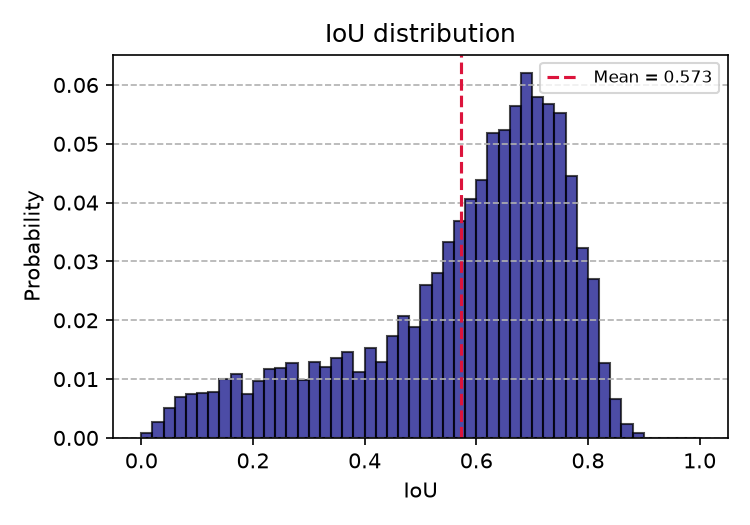
\includegraphics[width=0.49\linewidth]{oof1536_iou.png}\hfill
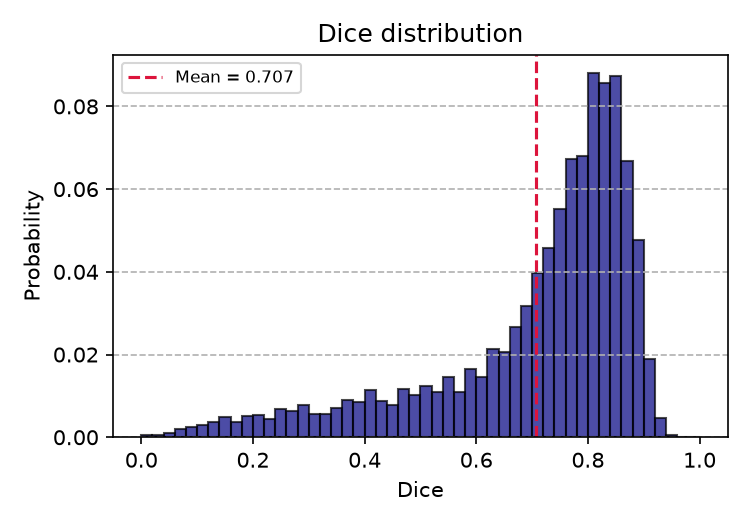
\includegraphics[width=0.49\linewidth]{oof1536_dice.png}\\[2pt]
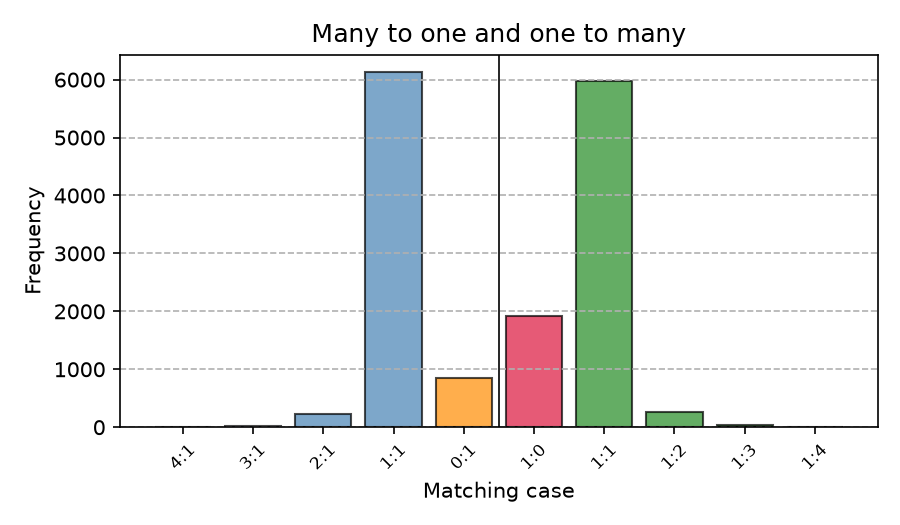
\includegraphics[width=0.9\linewidth]{oof1536_m2n.png}
\caption{Out-of-fold IoU and Dice distributions over GT/prediction pairs with IoU $>0$, and the
one-to-many / many-to-one counts (left: number of GT linked to each prediction; right: number of
predictions linked to each GT).}
\label{fig:dist}
\end{figure}

\begin{figure*}[t]
\centering
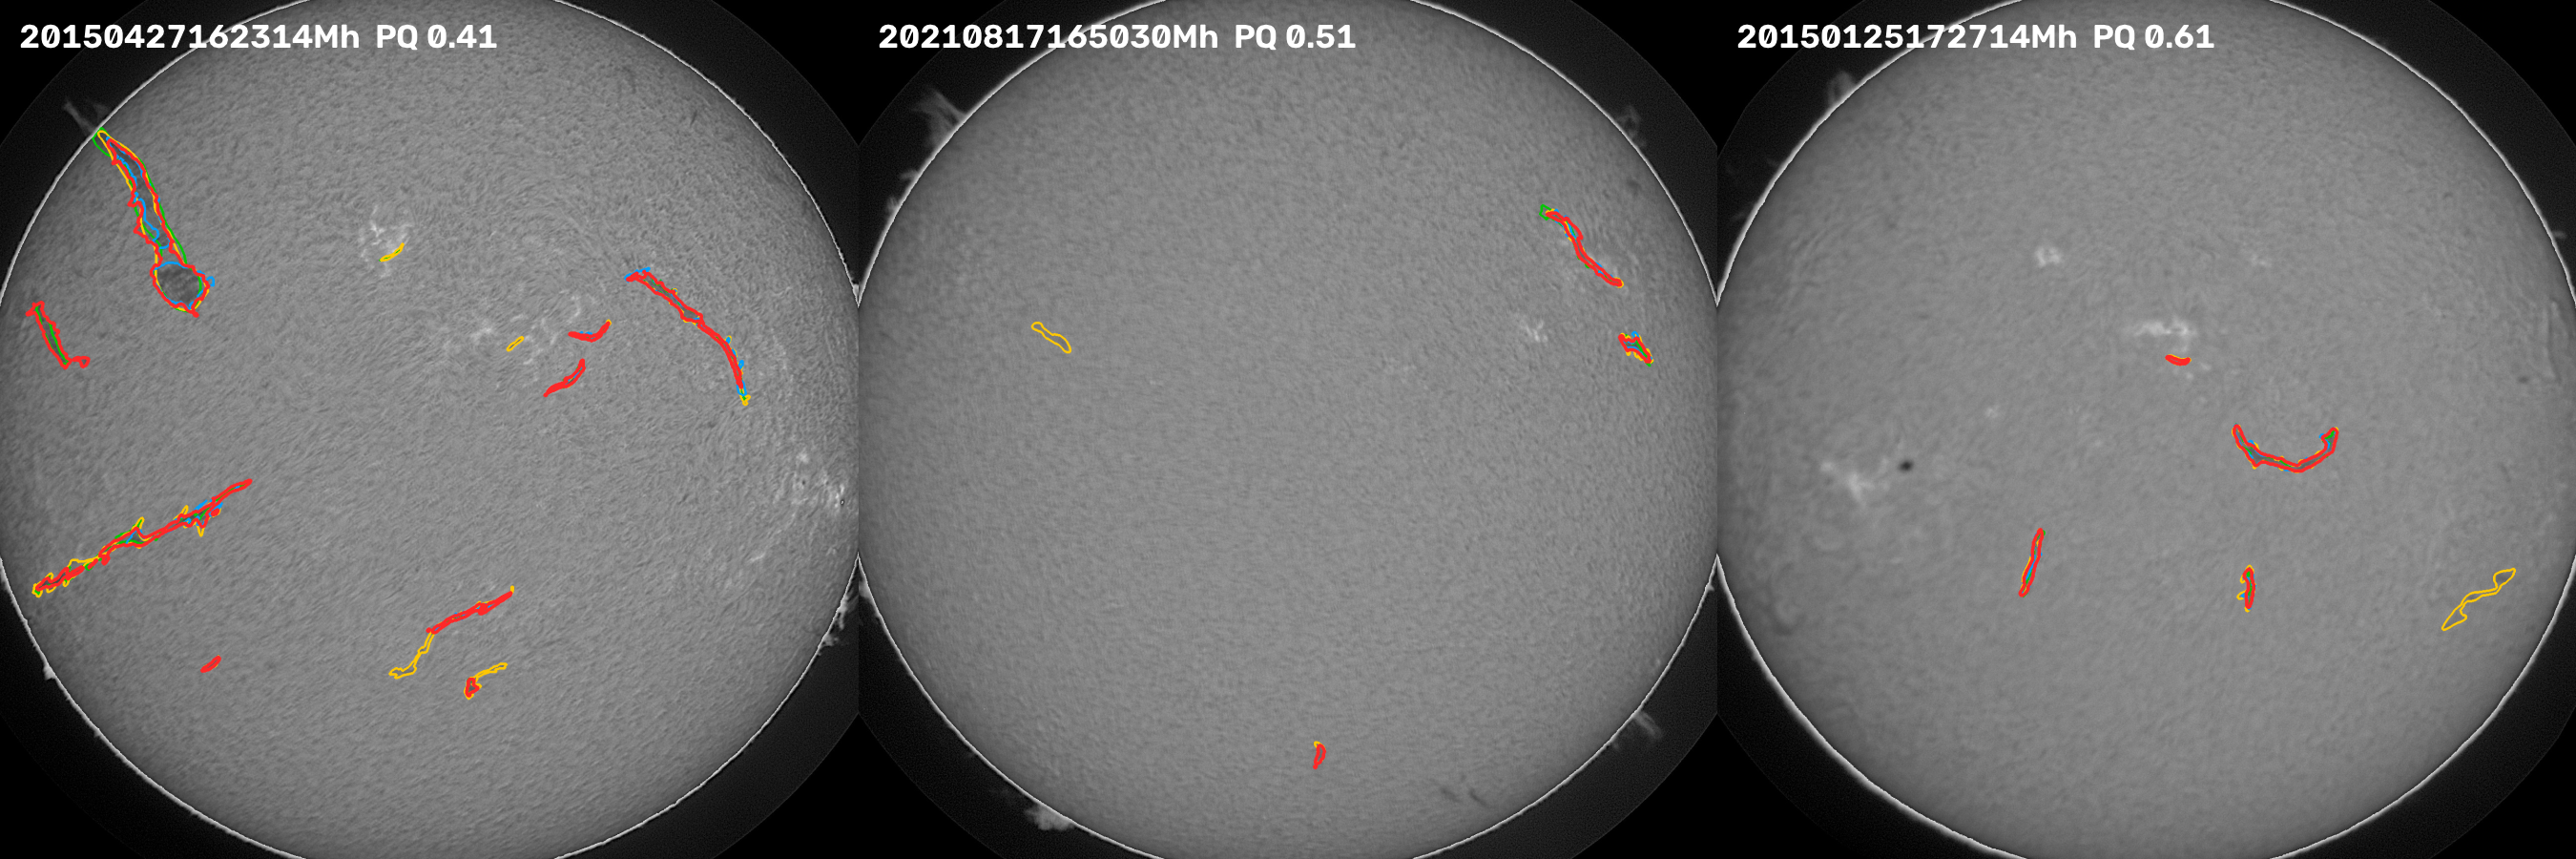
\includegraphics[width=\textwidth]{qualitative.png}
\caption{Out-of-fold predictions (red) on three validation images with three annotators (green, yellow,
blue), at the median, upper-quartile and near-best image PQ. Many misses are filaments marked by one
annotator only.}
\label{fig:qual}
\end{figure*}

\section{What did not help}
Table~\ref{tab:abl} lists the variants we tried, each evaluated with its own tuned post-processing.

\begin{table}[t]
\centering
\caption{Variants (fold 0, 142 images, tuned PQ) and post-processing rules (5-fold OOF, 707 images).}
\label{tab:abl}
\begin{tabular}{lc}
\toprule
Variant (fold 0) & PQ \\
\midrule
U-Net ResNet-34, 40 epochs (baseline) & \textbf{0.416} \\
\quad 10 / 20 epochs & 0.389 / 0.396 \\
\quad + crop refiner at native resolution & 0.413 \\
\quad + Mask R-CNN instances not covered by the U-Net & 0.417 \\
Mask R-CNN~\cite{maskrcnn} alone (disjoint masks) & 0.377 \\
ResNet-50 encoder & 0.414 \\
Limb-darkening-corrected input & 0.411 \\
BCE + Lov\'asz hinge~\cite{lovasz} & 0.390 \\
Average of ResNet-34 and ResNet-50 & 0.416 \\
\midrule
Post-processing rule (OOF) & PQ \\
\midrule
Submission setting (confidence $\geq 0.8$) & 0.409 \\
Confidence $\geq 0.85$ (reference for the rows below) & 0.411 \\
No closing, no confidence or limb filter & 0.398 \\
Size-dependent confidence threshold & 0.411 \\
Hysteresis (seed and grow thresholds) & 0.409 \\
8 dihedral views instead of 4 (fold 0) & 0.419 vs.\ 0.419 \\
2048~px input (folds 0, 3; default setting) & 0.404, 0.388 vs.\ 0.403, 0.387 \\
Masks dilated / eroded by 1~px & 0.381 / 0.399 \\
70-degree limb cut-off & no change \\
\bottomrule
\end{tabular}
\end{table}

\emph{Instance models.} A Mask R-CNN detector learns grouping explicitly, but its masks are coarser
(SQ 0.642 vs.\ 0.657 for a U-Net trained for a similar number of epochs) and it scores below the U-Net; adding its extra instances or a per-filament crop
refiner (following Reche \& Cid~\cite{reche2026}) changes PQ by less than 0.002 on the
fully trained U-Net.

\emph{Larger encoder, normalised input, IoU loss.} A ResNet-50 encoder, an input divided by its own
radial brightness profile (which also removes the scattered-light halo), and a Lov\'asz hinge loss all
match or underperform the baseline. With the corrected input the best threshold moves from 0.45 to 0.65:
the network becomes more confident, not more accurate.

\emph{Ensembles.} Averaging two equal-strength models with different encoders gives the same PQ as the
better one, and the 5-fold average gives the same leaderboard score as one model. The models share their
errors because the errors come from the annotators, so the final submission is one network.

\section{Where the remaining PQ is lost}\label{sec:loss}
\emph{Near misses.} Of the 3{,}174 OOF false negatives, 45\% overlap no prediction, 18\% overlap one at
IoU $<0.3$ and 37\% at IoU 0.3--0.5. Among the near misses the prediction is smaller than the GT in 46\% of
cases and larger in 34\%; only 17\% are merges with another filament and 16\% are splits. Dilating or
eroding every mask by a single pixel costs 0.01--0.03 PQ, because filaments are only a few pixels wide:
the extent errors are per instance, not a bias a rule could correct.

\emph{Small filaments.} Recall falls to 0.36 below 500~px. Annotators rarely agree on them: the share of
other annotators marking the same filament (IoU $>0.5$) is 0.28 below 300~px and about 0.60 above
1{,}000~px.

\emph{When a doubtful prediction pays.} A prediction matching $k$ of the $n$ annotators of an image adds
about $k\cdot\mathrm{IoU}$ to the numerator and $0.5n$ to the denominator, so it raises PQ only if
$k/n > \mathrm{PQ}/(2\,\mathrm{SQ}) \approx 0.31$. A filament marked by one annotator of three is break-even,
which is why lowering the area or confidence thresholds never helped; 28\% of our false positives match
another annotator's filament on the same image.

\section{Conclusion}
A consensus-trained U-Net at 1536~px with a learned component scorer gives OOF PQ 0.422 on MAGFiLO, above
the 0.340 that one annotator scores against another. Choosing instances by their expected contribution to
the metric helped more than any change to the segmenter; larger models, instance heads, input
normalisation, IoU losses, ensembling and hand post-processing rules did not, and the error analysis
attributes most of the remaining loss to disagreement between annotators. Further gains should come from modelling the
annotators (e.g.\ predicting each annotator's style) rather than from a stronger segmenter. Code, weights
and a notebook reproducing the submission are in the repository; every experiment is logged in
\texttt{docs/DESIGN.md}.

\begin{thebibliography}{9}
\bibitem{magfilo} A.~Ahmadzadeh \emph{et al.}, ``A dataset of manually annotated filaments from H-alpha observations,'' \emph{Scientific Data}, 2024, doi:10.1038/s41597-024-03876-y.
\bibitem{kirillov2019} A.~Kirillov, K.~He, R.~Girshick, C.~Rother, P.~Doll\'ar, ``Panoptic segmentation,'' in \emph{CVPR}, 2019.
\bibitem{unet} O.~Ronneberger, P.~Fischer, T.~Brox, ``U-Net: convolutional networks for biomedical image segmentation,'' in \emph{MICCAI}, 2015.
\bibitem{resnet} K.~He, X.~Zhang, S.~Ren, J.~Sun, ``Deep residual learning for image recognition,'' in \emph{CVPR}, 2016.
\bibitem{smp} P.~Iakubovskii, ``Segmentation Models Pytorch,'' GitHub repository, 2019.
\bibitem{maskrcnn} K.~He, G.~Gkioxari, P.~Doll\'ar, R.~Girshick, ``Mask R-CNN,'' in \emph{ICCV}, 2017.
\bibitem{lovasz} M.~Berman, A.~Rannen Triki, M.~B.~Blaschko, ``The Lov\'asz-softmax loss,'' in \emph{CVPR}, 2018.
\bibitem{reche2026} Reche and Cid, \emph{Acta Astronautica}, vol.~249, 2026.
\end{thebibliography}

\end{document}
